\section{Results} \label{results}

In this study, a single liquid slug segment within the ATC is simulated to investigate particle suspension behavior under representative operating conditions. The ATC's rotation is modeled by applying boundary conditions directly on the surface of the liquid slug mesh. Specifically, Dirichlet boundary conditions consistent with the rotational speed of the apparatus are imposed on the tube walls, while free-slip conditions are applied at the spherical gas–liquid interfaces at the slug ends. This setup replicates the internal recirculation patterns typical of Taylor vortices while incorporating the centrifugal effects that generate Dean vortices.
Particle transport within the slug is resolved using the two-way coupled DNS approach (see \ref{sec:modeling}). 

The ATC geometry simulated corresponds to a coiled tube with a diameter of $d_{ct} = 50\,\text{mm}$, consistent with the experimental setup described in prior validation work (see also Figure \ref{Setup}). 
Simulations are performed across a range of ATC rotational speeds ($n_\mathrm{ATC}$) to match experimental conditions designed to generate different flow regimes. The configuration of the cases is summarized in Table \ref{tab:allcases}, while a list of fluid and particle properties can be found in Table \ref{tab:exp_op_points:properties}.

\begin{table}[H]
    \centering
    \caption{Summary of DNS simulation setup and cases, ordered by flow map zone. All simulations use \textsc{l}-alanine particles suspended in an aqueous solution. Cases are defined by varying rotational speed, particle diameter, and solid content at a constant filling degree of $\varepsilon$ = 0.25.}
    \label{tab:allcases}
    \begin{tabular}{ccccc}
        \toprule
        Case ID & $n_\text{ATC}$ [rpm] & $d_p$ [$\mu$m] & $w_\mathrm{solid}$ [wt\%] & Flow Map Zone \\
        \midrule
        C1 & 40 & 182 & 1.0 & green \\
        C2 & 40 & 182 & 5.1 & green \\
        C3 & 40 & 273 & 1.0 & yellow \\
        C4 & 40 & 273 & 5.1 & yellow \\
        C5 & 25 & 273 & 1.0 & red/yellow \\
        C6 & 25 & 273 & 5.1 & red/yellow \\
        C7 & 12 & 364 & 1.0 & red \\
        C8 & 12 & 364 & 5.1 & red \\
        \bottomrule
    \end{tabular}
\end{table}

First, the simulation results are compared directly to experimental observations using side-view imaging (see Figure \ref{fig:image_comp_all}) of particle distribution within the ATC, as explained in section \ref{sec::experimenalSetup}. Secondly, the quantitative evaluation using the metrics defined in section \ref{sec:metricSection} validate the simulation approach, demonstrating that the two-way coupled DNS framework reliably predicts suspension states across the experimentally observed flow regimes. This integrated validation ensures that the simulated flow fields and suspension patterns correspond realistically to those observed in the laboratory, supporting the predictive use of the model for design and optimization of ATC operation. 

\subsection{Qualitative Comparison with Experimental Data}
\begin{figure}[H]

  \centering
  \includegraphics[width=\textwidth]{Figures/Fig4a.png}

  \caption{Comparison for cases C1, C2, C3, and C4. C1 and C2 reprinted from \cite{Sonnenschein.2021}. Copyright CC BY 4.0}
  \label{fig:image_comp_all}
\end{figure}

\begin{figure}[H]
  \centering
  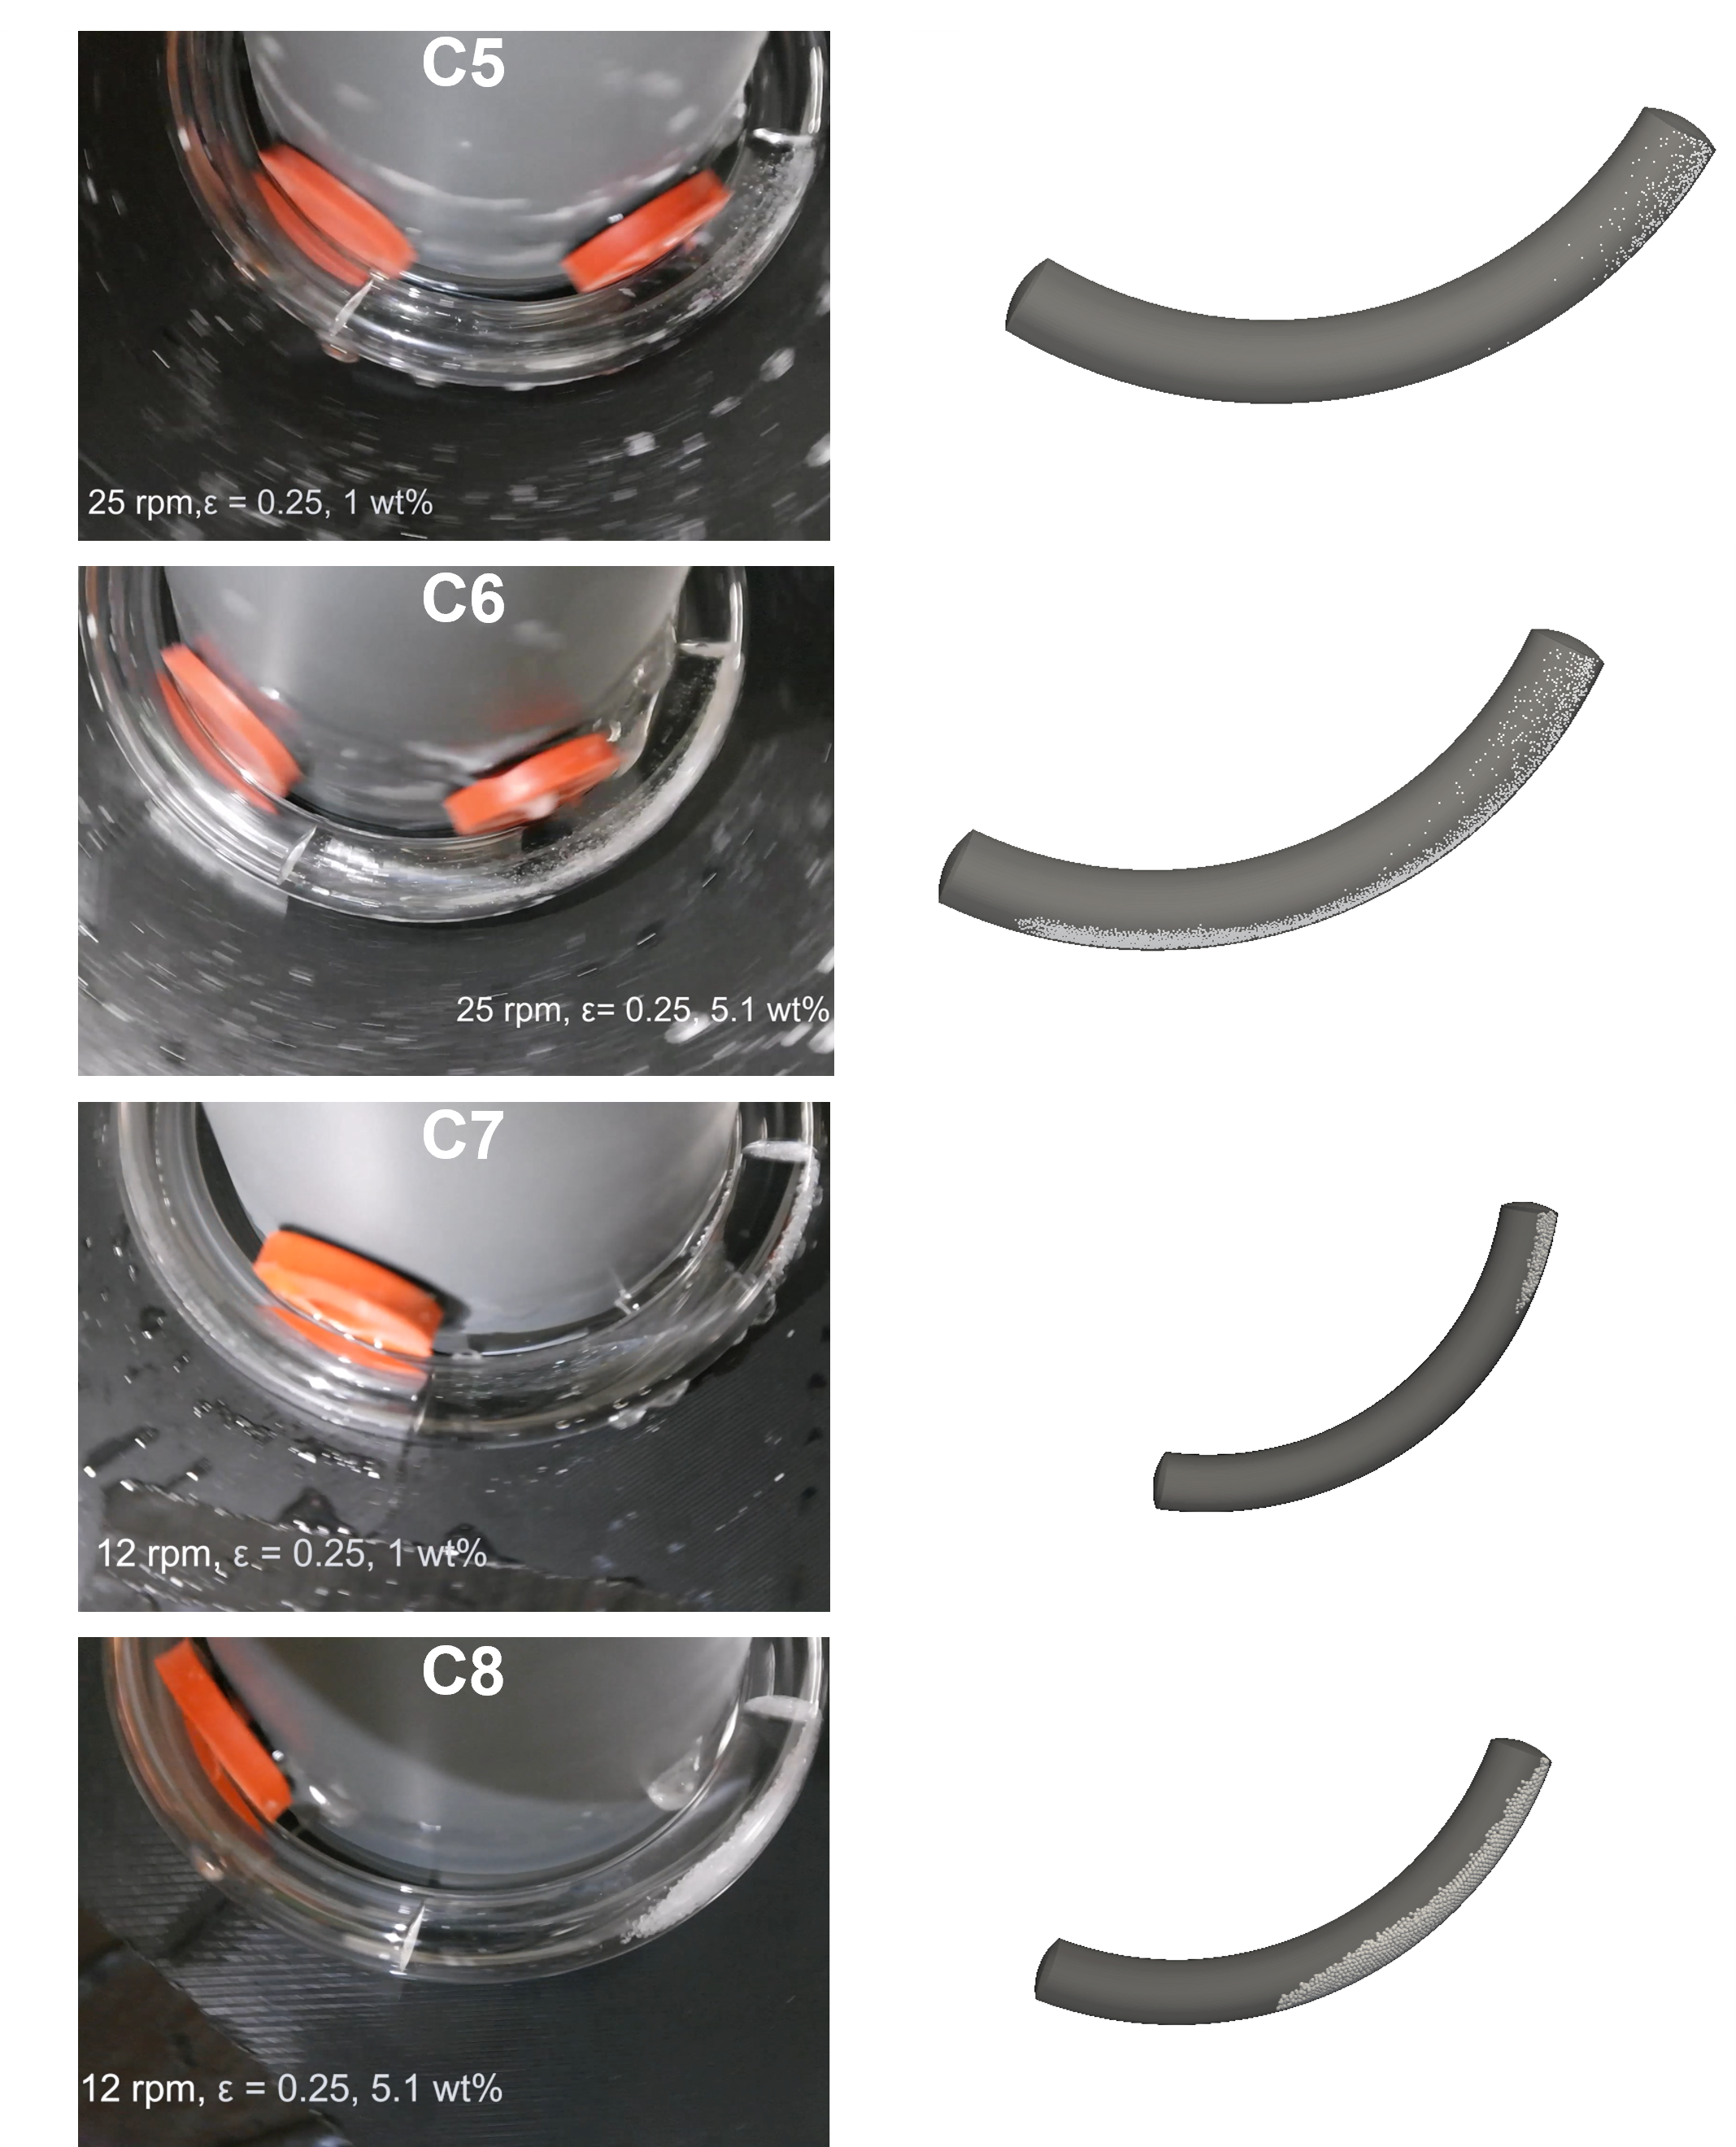
\includegraphics[width=\textwidth]{Figures/Fig5a.png}

  \caption{Comparison for cases C5, C6, C7, and C8.}
\end{figure}

\subsection{Metric-based Quantitative Analysis}

% First four cases
\begin{figure}[H]
    \centering
    \begin{subfigure}[b]{0.48\textwidth}
        \includegraphics[width=\textwidth]{Figures/case1_axial_distribution.png}
        \caption{Case C1}
    \end{subfigure}\hfill
    \begin{subfigure}[b]{0.48\textwidth}
        \includegraphics[width=\textwidth]{Figures/case2_axial_distribution.png}
        \caption{Case C2}
    \end{subfigure}

    \vspace{1em}

    \begin{subfigure}[b]{0.48\textwidth}
        \includegraphics[width=\textwidth]{Figures/case3_axial_distribution.png}
        \caption{Case C3}
    \end{subfigure}\hfill
    \begin{subfigure}[b]{0.48\textwidth}
        \includegraphics[width=\textwidth]{Figures/case4_axial_distribution.png}
        \caption{Case C4}
    \end{subfigure}
    \caption{Axial particle distribution $\overline{\phi}(z)$ for cases C1–C4.}
    \label{fig:axial_distribution_1_4}
\end{figure}

% Next four cases
\begin{figure}[H]
    \centering
    \begin{subfigure}[b]{0.48\textwidth}
        \includegraphics[width=\textwidth]{Figures/case5_axial_distribution.png}
        \caption{Case C5}
    \end{subfigure}\hfill
    \begin{subfigure}[b]{0.48\textwidth}
        \includegraphics[width=\textwidth]{Figures/case6_axial_distribution.png}
        \caption{Case C6}
    \end{subfigure}

    \vspace{1em}

    \begin{subfigure}[b]{0.48\textwidth}
        \includegraphics[width=\textwidth]{Figures/case7_axial_distribution.png}
        \caption{Case C7}
    \end{subfigure}\hfill
    \begin{subfigure}[b]{0.48\textwidth}
        \includegraphics[width=\textwidth]{Figures/case8_axial_distribution.png}
        \caption{Case C8}
    \end{subfigure}
    \caption{Axial particle distribution $\overline{\phi}(z)$ for cases C5–C8.}
    \label{fig:axial_distribution_5_8}
\end{figure}

\clearpage
%\subsection{Radial Distribution Index $I_r$}

% First four cases
\begin{figure}[H]
    \centering
    \begin{subfigure}[b]{0.48\textwidth}
        \includegraphics[width=\textwidth]{Figures/case_1_equal_area_equal_area_radial_analysis.png}
        \caption{Case C1}
    \end{subfigure}\hfill
    \begin{subfigure}[b]{0.48\textwidth}
        \includegraphics[width=\textwidth]{Figures/case_2_equal_area_equal_area_radial_analysis.png}
        \caption{Case C2}
    \end{subfigure}

    \vspace{1em}

    \begin{subfigure}[b]{0.48\textwidth}
        \includegraphics[width=\textwidth]{Figures/case_3_equal_area_equal_area_radial_analysis.png}
        \caption{Case C3}
    \end{subfigure}\hfill
    \begin{subfigure}[b]{0.48\textwidth}
        \includegraphics[width=\textwidth]{Figures/case_4_equal_area_equal_area_radial_analysis.png}
        \caption{Case C4}
    \end{subfigure}
    \caption{Equal-area radial distribution analysis for cases C1–C4.}
    \label{fig:radial_distribution_1_4}
\end{figure}

\clearpage
% Next four cases
\begin{figure}[H]
    \centering
    \begin{subfigure}[b]{0.48\textwidth}
        \includegraphics[width=\textwidth]{Figures/case_5_equal_area_equal_area_radial_analysis.png}
        \caption{Case C5}
    \end{subfigure}\hfill
    \begin{subfigure}[b]{0.48\textwidth}
        \includegraphics[width=\textwidth]{Figures/case_6_equal_area_equal_area_radial_analysis.png}
        \caption{Case C6}
    \end{subfigure}

    \vspace{1em}

    \begin{subfigure}[b]{0.48\textwidth}
        \includegraphics[width=\textwidth]{Figures/case_7_equal_area_equal_area_radial_analysis.png}
        \caption{Case C7}
    \end{subfigure}\hfill
    \begin{subfigure}[b]{0.48\textwidth}
        \includegraphics[width=\textwidth]{Figures/case_8_equal_area_equal_area_radial_analysis.png}
        \caption{Case C8}
    \end{subfigure}
    \caption{Equal-area radial distribution analysis for cases C5–C8.}
    \label{fig:radial_distribution_5_8}
\end{figure}

\begin{comment}
\subsubsection{Interpretation of axial and radial metrics.}
The axial profiles $\overline{\phi}(z)$ and the equal‑area radial analysis together clarify the regime transitions:

\begin{itemize}
  \item \textbf{Green (C1–C2):} Very high $I_r$ ($\approx 0.90$) corresponds to genuinely uniform cross‑sectional mixing. 
  The \emph{front} of the slug is notably populated and the \emph{middle radial bins} are well filled—both signatures of a robust two‑vortex structure and efficient Dean–Taylor recirculation.

  \item \textbf{Yellow (C3–C4):} $I_r$ drops to $0.77$ (C3) and $0.57$ (C4). We observe the onset of radial inhomogeneity:
  the \emph{middle bins begin to depopulate}, and the \emph{front} receives markedly fewer particles. This is consistent with a weakened upper vortex and increasing gravitational bias.

  \item \textbf{Red/Yellow (C5–C6):} Further decline in $I_r$ (down to $0.41$ in C6) reflects pronounced wall/bottom accumulation and rear loading in $\overline{\phi}(z)$. 
  The \emph{middle bins are largely left empty}, and the front remains sparsely populated.

  \item \textbf{Red (C7–C8):} Although $I_r$ is \emph{slightly higher} than C6 ($0.48$ and $0.47$ vs.\ $0.41$), \textbf{this is not an improvement in mixing}. 
  It results from \textbf{rear loading followed by stacking} in the back of the slug: particles gather and layer radially in a compact region. 
  In the equal‑area binning, the \textbf{larger particle size} (364\,$\mu$m) also occupies more bins geometrically, which can inflate $I_r$ even when the distribution is not truly uniform. 
  The \emph{front} remains nearly unpopulated and the \emph{middle bins stay depleted}, so the physical picture is still a gravity‑dominated, poorly mixed state.
\end{itemize}

\subsubsection{Distinctive trends across regimes.}
\begin{enumerate}
  \item \textbf{Middle radial bins empty quickly outside green:} As soon as we leave the green zone, the equal‑area analysis shows a rapid depletion of \emph{middle} bins, indicating collapse toward wall/bottom regions and loss of cross‑sectional uniformity.
  \item \textbf{Front population is a hallmark of green:} Only in the green regime do particles significantly populate the \emph{front} of the slug, reflecting strong, balanced secondary vortices that transport particles throughout the compartment.
\end{enumerate}

\subsubsection{Vertical Asymmetry}
The vertical asymmetry metric $A_y$ complements the axial particle distribution $\overline{\phi}(z)$ and radial distribution index $I_r$ by explicitly quantifying the partitioning of solids between the upper and lower halves of the tube cross-section.

In the \textbf{green flow map regime} (C1–C2, 40\,rpm, $d_p=182\,\mu$m), $A_y$ remains close to zero ($0.020$ for C1, $-0.119$ for C2), indicating near-symmetric vertical suspension. This symmetry, combined with high $I_r$ values ($\approx 0.90$) and axial profiles showing both front and rear populations, reflects strong, balanced Dean vortices that counteract gravity effectively. The slight negative shift for C2 is attributed to the increased solids loading (5.1\,wt\%), which mildly suppresses vertical transport despite maintaining high radial uniformity.

\begin{figure} [h]
    \centering
    \includegraphics[width=0.5\textwidth]{Figures/C3_ay.png}
    \caption{Fluid Domain with middle surface visualization: Even though the yellow flow regime clearly exhibits vortex-driven dynamics the influence of the vortices is not enough to populate the upper half of the domain significantly.}
    \label{fig:case3_ay}
\end{figure}

In the \textbf{yellow regime} (C3–C4, 40\,rpm, $d_p=273\,\mu$m), $A_y$ plunges to $-0.976$ and $-0.878$, signifying that almost all particles reside in the lower half of the cross-section (see fig. \ref{fig:case3_ay}). Notably, $I_r$ values (0.77 for C3, 0.57 for C4) suggest substantial radial spread \emph{within} this lower half. Axially, these cases show rear-loading and depopulated front regions, consistent with diminished upper-vortex activity.

The \textbf{red/yellow regime} (C5–C6, 25\,rpm, $d_p=273\,\mu$m) exhibits a similar bottom dominance ($A_y \approx -0.95$) alongside lower $I_r$ (0.54 and 0.41), indicating both strong gravitational settling and reduced radial mixing. The axial profiles reveal pronounced rear concentration, while the equal-area radial analysis shows rapid depletion of the middle bins once the green regime is left.

Finally, in the \textbf{red regime} (C7–C8, 12\,rpm, $d_p=364\,\mu$m), $A_y = -1.000$ confirms that all particles are located below the mid-plane. The moderate $I_r$ values ($\approx 0.47$) here do not reflect improved mixing; instead, they arise from \emph{rear loading followed by stacking} in the lower rear of the slug. The larger particles also geometrically occupy more equal-area radial bins, which can artificially raise $I_r$ without any true vertical homogenization. The front of the slug remains entirely unpopulated in these cases.

Overall, $A_y$ reveals that meaningful upper-half particle population and front-filling occur \emph{only} in the green regime. Leaving this regime leads to rapid loss of vertical symmetry, depletion of the middle radial bins, and gravitationally dominated stacking at the rear of the slug, even when $I_r$ alone might suggest partial uniformity.

The agreement between DNS and experiment across multiple suspension states demonstrates the predictive capability of the method. We conclude by discussing its implications for ATC design and pointing out future directions toward higher particle numbers and closure development.
\end{comment}

\subsubsection{Analysis and Interpretation of Metric Evaluations}

The three quantitative descriptors---axial distribution $\phi(z)$ (see Figures \ref{fig:axial_distribution_1_4}, \ref{fig:axial_distribution_5_8}), radial index $I_r$ (see Figures \ref{fig:radial_distribution_1_4}, \ref{fig:radial_distribution_5_8}), and vertical asymmetry $A_y$---together provide a consistent picture of the suspension regimes across all simulated cases (see Table~\ref{tab:Ir_Ay_values}). By considering these metrics in combination rather than isolation, the distinct transitions between green, yellow, red/yellow, and red flow map zones can be interpreted with greater clarity.
    

In the \textbf{green regime} (C1--C2), the axial profiles are nearly flat, indicating homogeneous axial distributions. The radial index reaches very high values ($I_r \approx 0.90$), reflecting a uniform cross-sectional spread, while the asymmetry remains close to zero ($A_y = 0.020$ and $-0.119$). Together, these values confirm that particles are well suspended by balanced Dean vortices that counteract gravitational settling. Slight deviations in $A_y$ at higher solid content (C2) suggest mild bottom-heaviness, but radial and axial homogeneity remain largely intact.

\begin{figure} [h]
    \centering
    \includegraphics[width=0.5\textwidth]{Figures/C3_ay.png}
    \caption{Fluid Domain with middle surface visualization: Even though the yellow flow regime clearly exhibits vortex-driven dynamics the influence of the vortices is not enough to populate the upper half of the domain significantly.}
    \label{fig:case3_ay}
\end{figure}

Moving into the \textbf{yellow regime} (C3--C4), the metrics shift markedly. The axial profiles show rear-loading and depleted fronts, while $I_r$ decreases to 0.77 (C3) and 0.57 (C4), indicating loss of cross-sectional uniformity. Simultaneously, $A_y$ plunges close to $-1$, confirming that particles overwhelmingly reside in the lower half of the tube (see Figure \ref{fig:case3_ay}). This joint trend reveals the collapse of upper-vortex activity and the emergence of strong gravitational bias, with only partial radial spreading persisting within the bottom half.

The \textbf{red/yellow regime} (C5--C6) continues this progression. The axial distribution becomes increasingly rear-biased, $I_r$ falls further (0.54 and 0.41), and $A_y \approx -0.95$ shows that vertical symmetry is almost entirely lost. In this state, particles not only settle toward the bottom but also accumulate strongly at the rear, consistent with stacking and poor recirculation. The middle radial bins are nearly empty, underscoring the breakdown of cross-sectional mixing once the green regime is left.

Finally, in the \textbf{red regime} (C7--C8), all three metrics confirm a gravity-dominated state. The axial profiles exhibit extreme rear loading, and $A_y = -1.000$ indicates that all particles are below the mid-plane. While the value of $I_r$ ($\approx 0.47$) appears moderate, it is misleading. It arises from geometric binning effects due to rear stacking, rather than from genuine radial uniformity. The front of the slug remains unpopulated, and the suspension effectively collapses into a dense, bottom-heavy cluster.

Taken together, these results demonstrate that meaningful upper-half particle population and front-filling occur only in the green regime. Exiting this regime leads to rapid depletion of the middle radial bins, progressive rear-loading, and strong vertical asymmetry.
Interpreting jointly $\phi(z)$, $I_r$, and $A_y$ is essential. For example, the moderately high $I_r$ in C7–C8 suggests partial uniformity, yet the combination of metrics (see Table~\ref{tab:Ir_Ay_values}) reveals the true, gravity-dominated state.  

\begin{table}[H]
\centering
\caption{Axial particle distribution $\overline{\phi}(z)$, radial distribution index $I_r$, and vertical asymmetry index $A_y$ 
for all simulated cases. A nearly flat $\overline{\phi}(z)$ profile indicates homogeneous axial distribution, while rear-loading 
or mid/rear peaks indicate segregation. Higher $I_r$ corresponds to a more uniform radial spread. 
$A_y \approx 0$ indicates vertical symmetry; $A_y < 0$ reflects bottom-heavy configurations; 
$A_y = -1$ corresponds to all particles below the mid-plane.}
\label{tab:Ir_Ay_values}
\begin{tabular}{lcccccc}
\toprule
Case & $\overline{\phi}(z)$ & $I_r$ & $A_y$ & $\phi_{\mathrm{upper}}$ & $\phi_{\mathrm{lower}}$ & Flow Map Zone \\
\midrule
C1 & nearly flat        & 0.9114 &  0.0198 & 0.5099 & 0.4901 & green \\
C2 & nearly flat        & 0.8992 & -0.1188 & 0.4406 & 0.5594 & green \\
C3 & mid–rear           & 0.7664 & -0.9764 & 0.0118 & 0.9882 & yellow \\
C4 & mid–rear           & 0.5657 & -0.8780 & 0.0610 & 0.9390 & yellow \\
C5 & rear-biased        & 0.5372 & -0.9597 & 0.0202 & 0.9798 & red/yellow \\
C6 & rear-biased        & 0.4056 & -0.9453 & 0.0273 & 0.9727 & red/yellow \\
C7 & rear-loaded        & 0.4767 & -1.0000 & 0.0000 & 1.0000 & red \\
C8 & rear-loaded        & 0.4720 & -1.0000 & 0.0000 & 1.0000 & red \\
\bottomrule
\end{tabular}
\end{table}
